Die Proximety-App setzt auf eine Client-Server-Architektur. 

Auf dem mobilen Gerät - dem Client - ist das User-Interface (GUI) zu finden. Alle Interaktionen, welche mit dem Benutzer stattfinden sind auf dem mobilen Gerät zu finden.

Auf dem Server sind Services vorhanden, welche die Daten der App in einer Datenbank persistieren. Zusätzlich wird auf dem Server periodisch die Distanz zwischen den einzelnen Freunden berechnet und an die betroffenen Client gepusht.

\subsection{Klassendiagramm App}
Das Klassendiagramm in Abbildung~\ref{fig:Proximety_Classes} beinhaltet alle Klassen, welche auf Android - als auf der Seite des mobilen Gerätes - gebraucht werden.
\FloatBarrier
\begin{figure}[H]
	\centering
		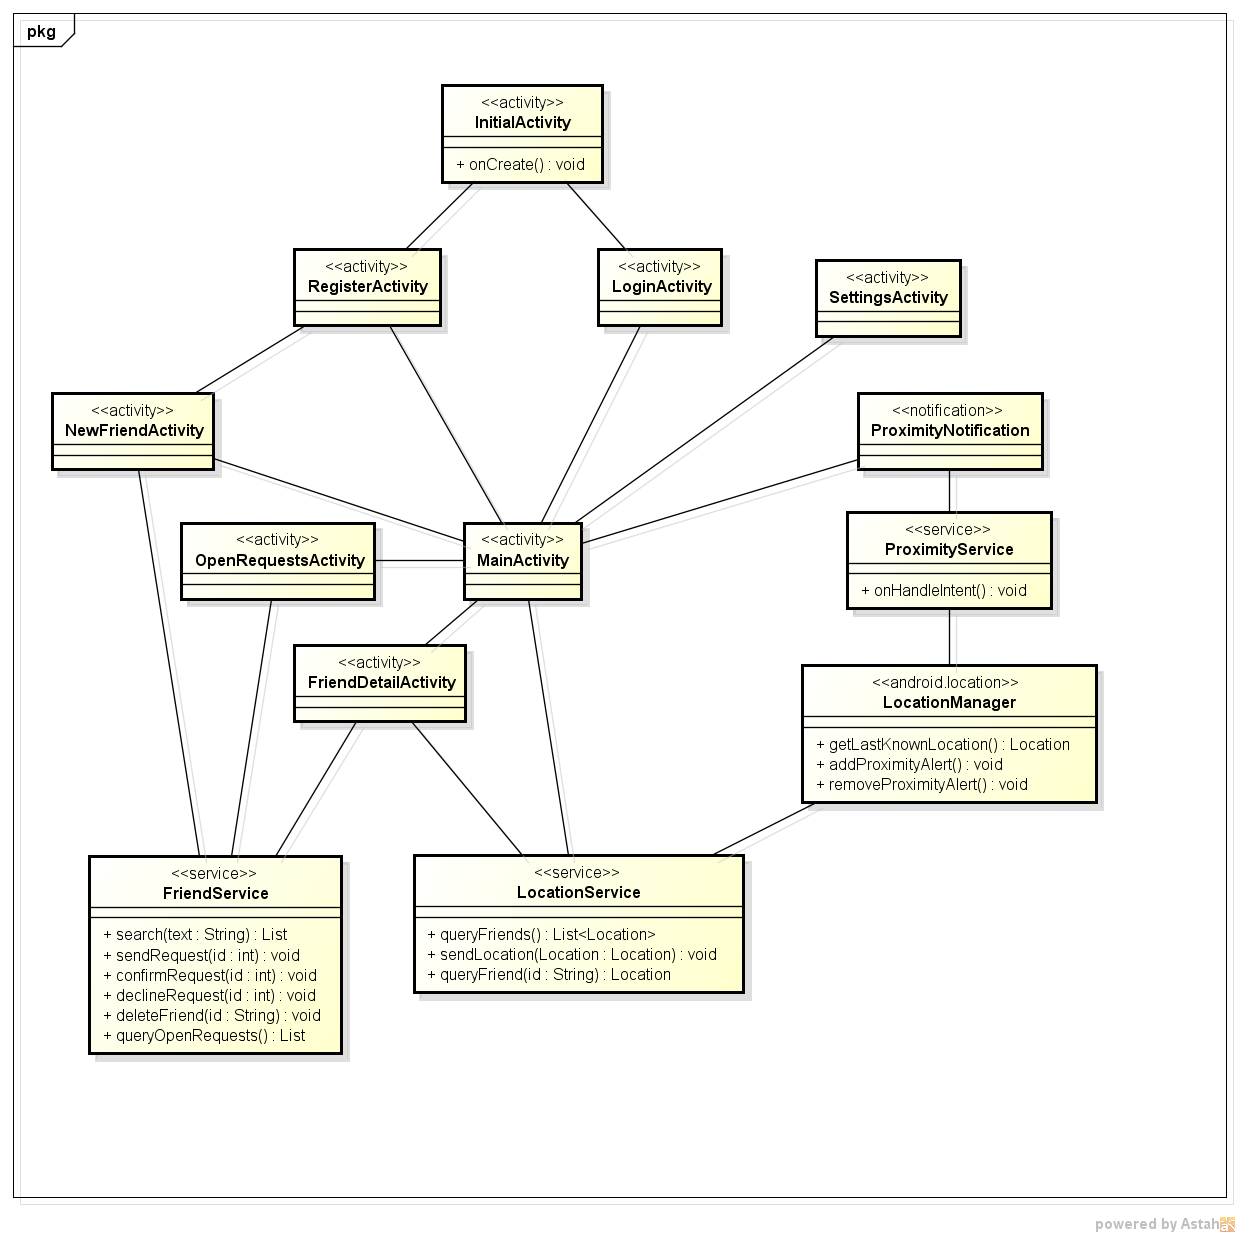
\includegraphics[width=\textwidth]{architektur/Proximety_Classes}
	\caption{Klassendiagramm der App}
	\label{fig:Proximety_Classes}
\end{figure}

\FloatBarrier
\subsection{Klassendiagramm Server}
Das Klassendiagramm in Abbildung~\ref{fig:Proximety_Server_Classes} beinhaltet alle Klassen, welche auf dem Server gebraucht werden.
\begin{figure}[H]
	\centering
		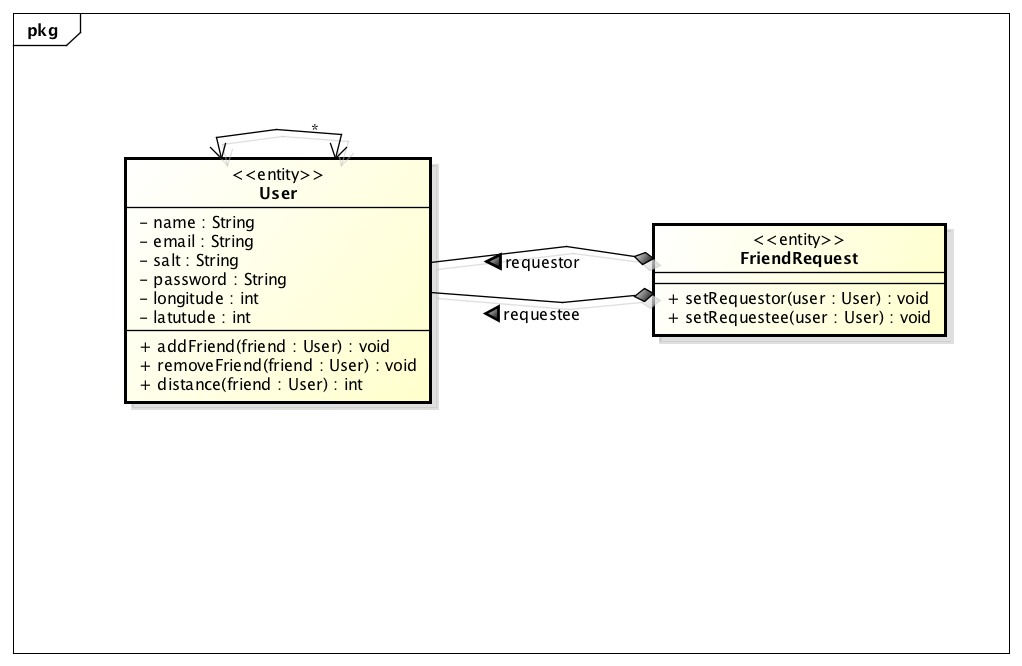
\includegraphics[width=\textwidth]{architektur/Proximety_Server_Classes}
	\caption{Klassendiagramm des Server}
	\label{fig:Proximety_Server_Classes}
\end{figure}

\FloatBarrier
\subsection{Sequenzdiagramm Startup-Sequenz}
Das Sequenzdiagramm in Abbildung~\ref{fig:Proximety_Startup_Sequence_Diagram} visualisiert den Prozess, welcher ein Benutzer durchläuft, wenn er die App zum ersten Mal startet.
\begin{figure}[H]
	\centering
		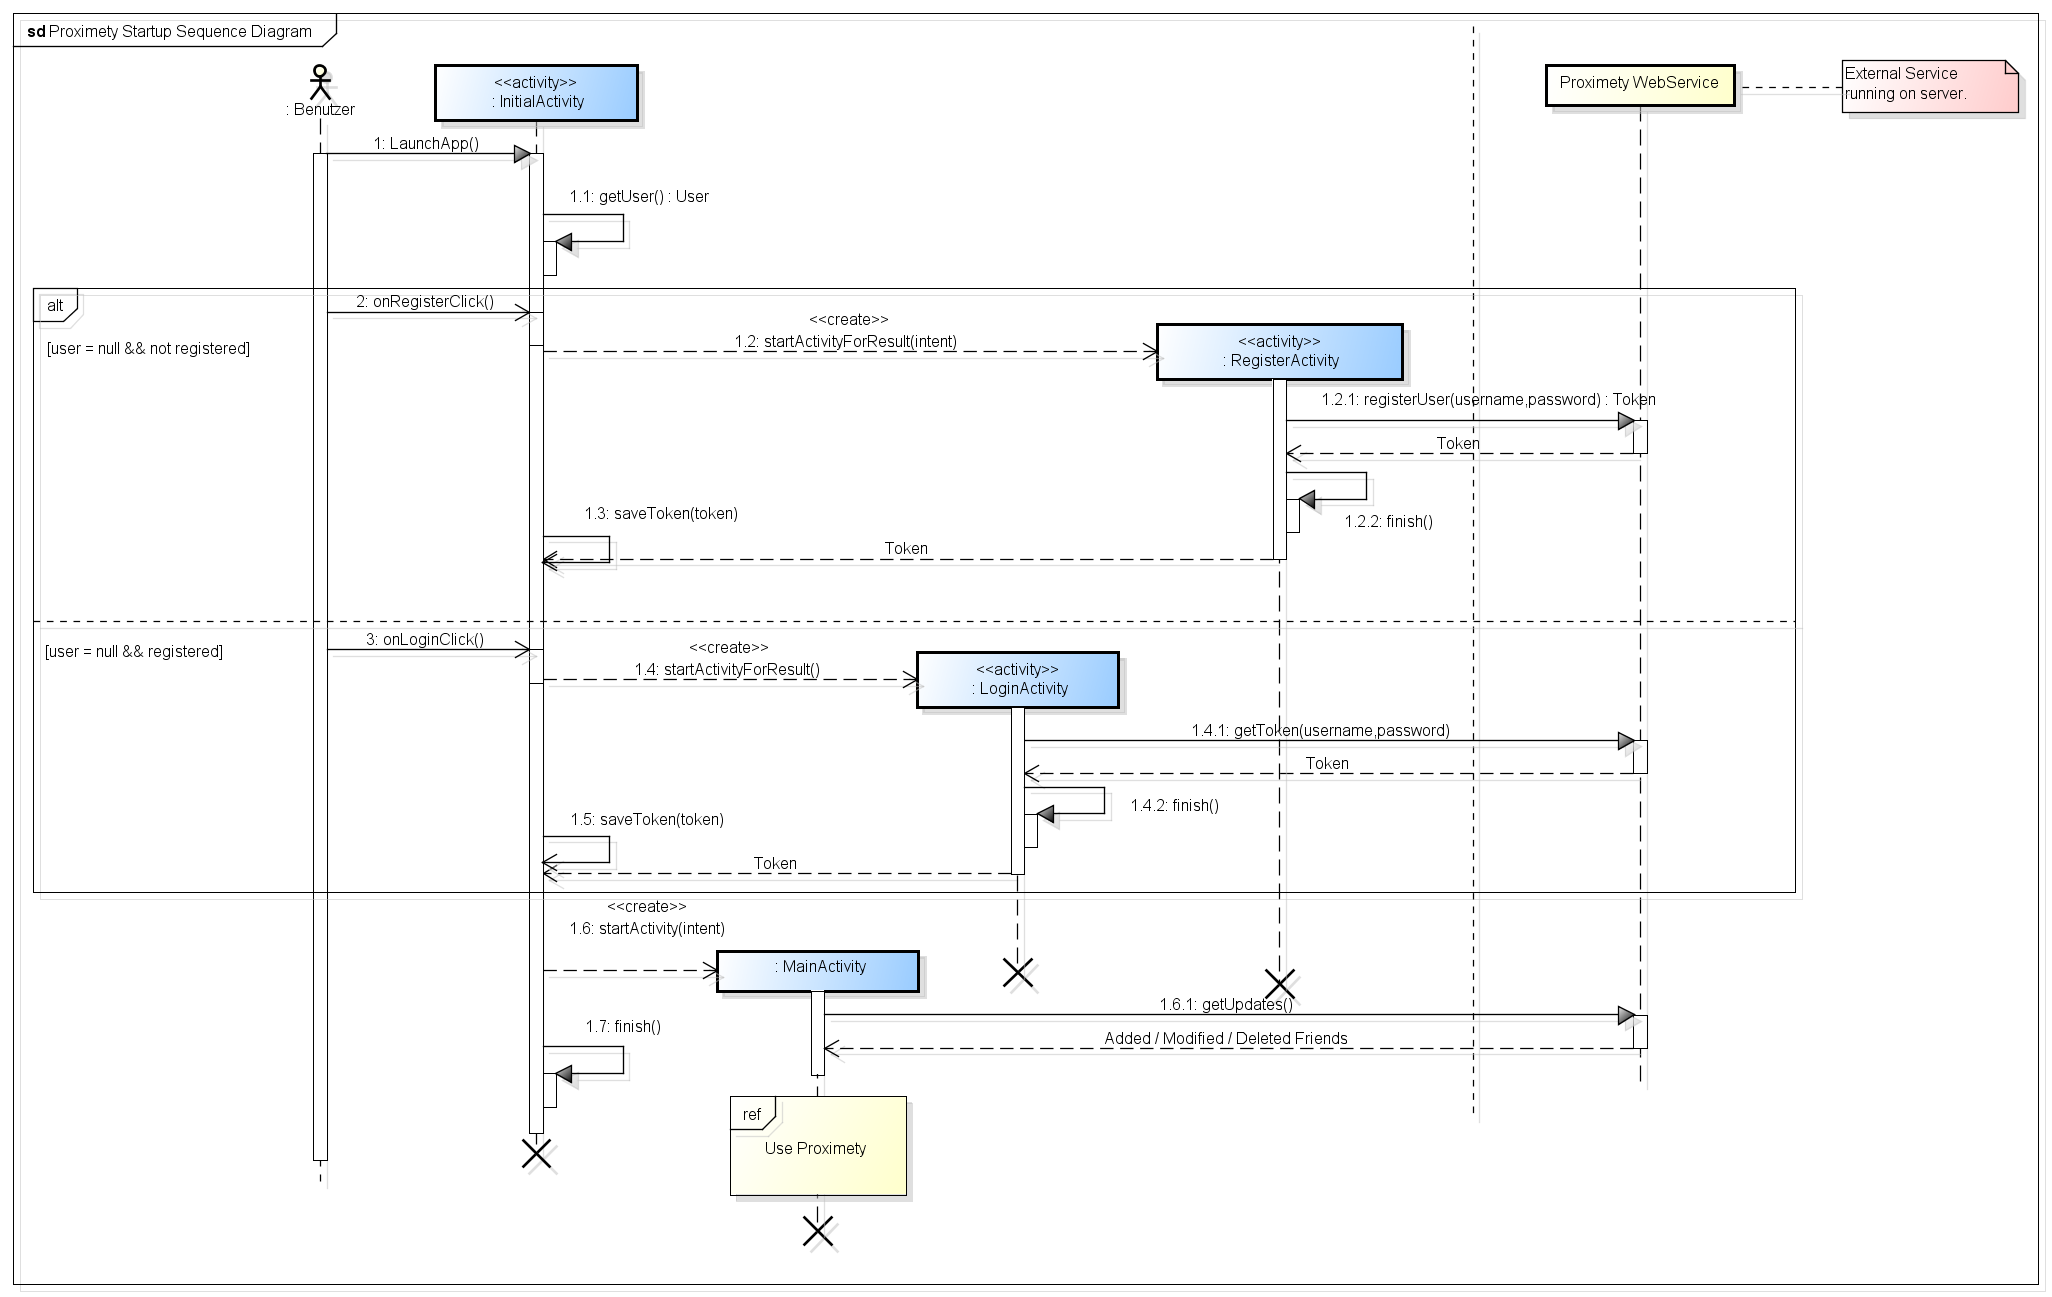
\includegraphics[width=\textwidth]{architektur/Proximety_Startup_Sequence_Diagram}
	\caption{Sequenzdiagramm Startup-Sequenz}
	\label{fig:Proximety_Startup_Sequence_Diagram}
\end{figure}

\FloatBarrier
\subsection{Sequenzdiagramm Account registrieren}
Das Sequenzdiagramm in Abbildung~\ref{fig:UC01_Account_registrieren} visualisiert den Prozess, welcher in UC01 beschrieben ist.
\begin{figure}[H]
	\centering
		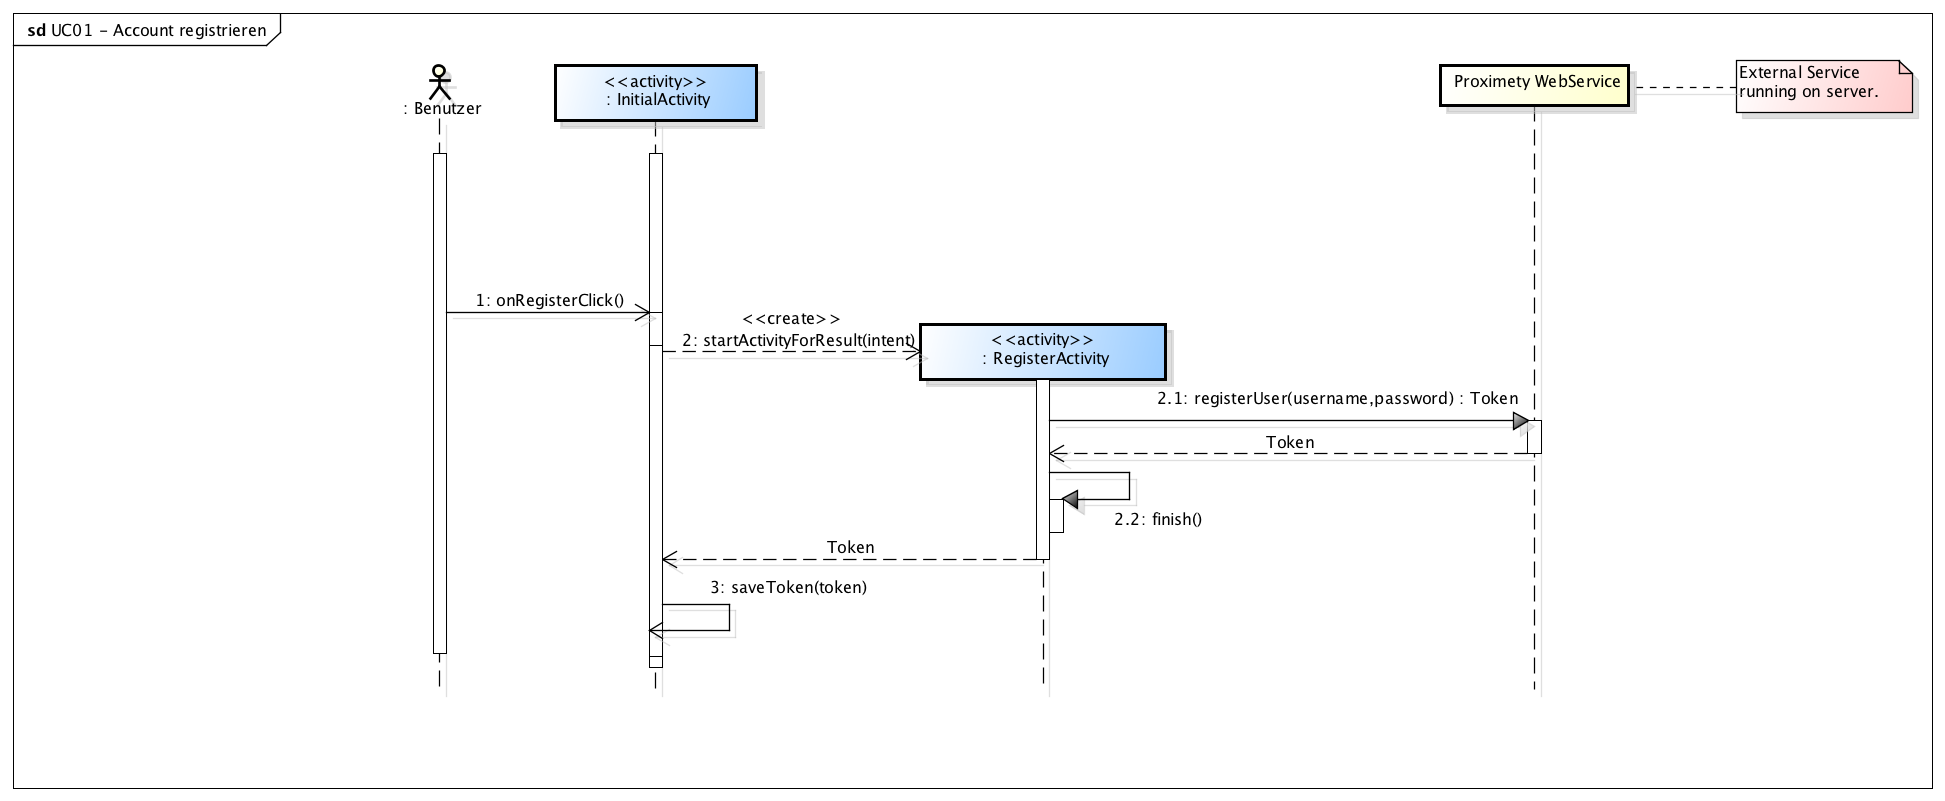
\includegraphics[width=\textwidth]{architektur/UC01_Account_registrieren}
	\caption{Sequenzdiagramm Account registrieren}
	\label{fig:UC01_Account_registrieren}
\end{figure}

\FloatBarrier
\subsection{Sequenzdiagramm Freundschaftsanfrage versenden}
Das Sequenzdiagramm in Abbildung~\ref{fig:UC02_Freundschaftsanfrage_versenden} visualisiert den Prozess, welcher in UC02 beschrieben ist.
\begin{figure}[H]
	\centering
		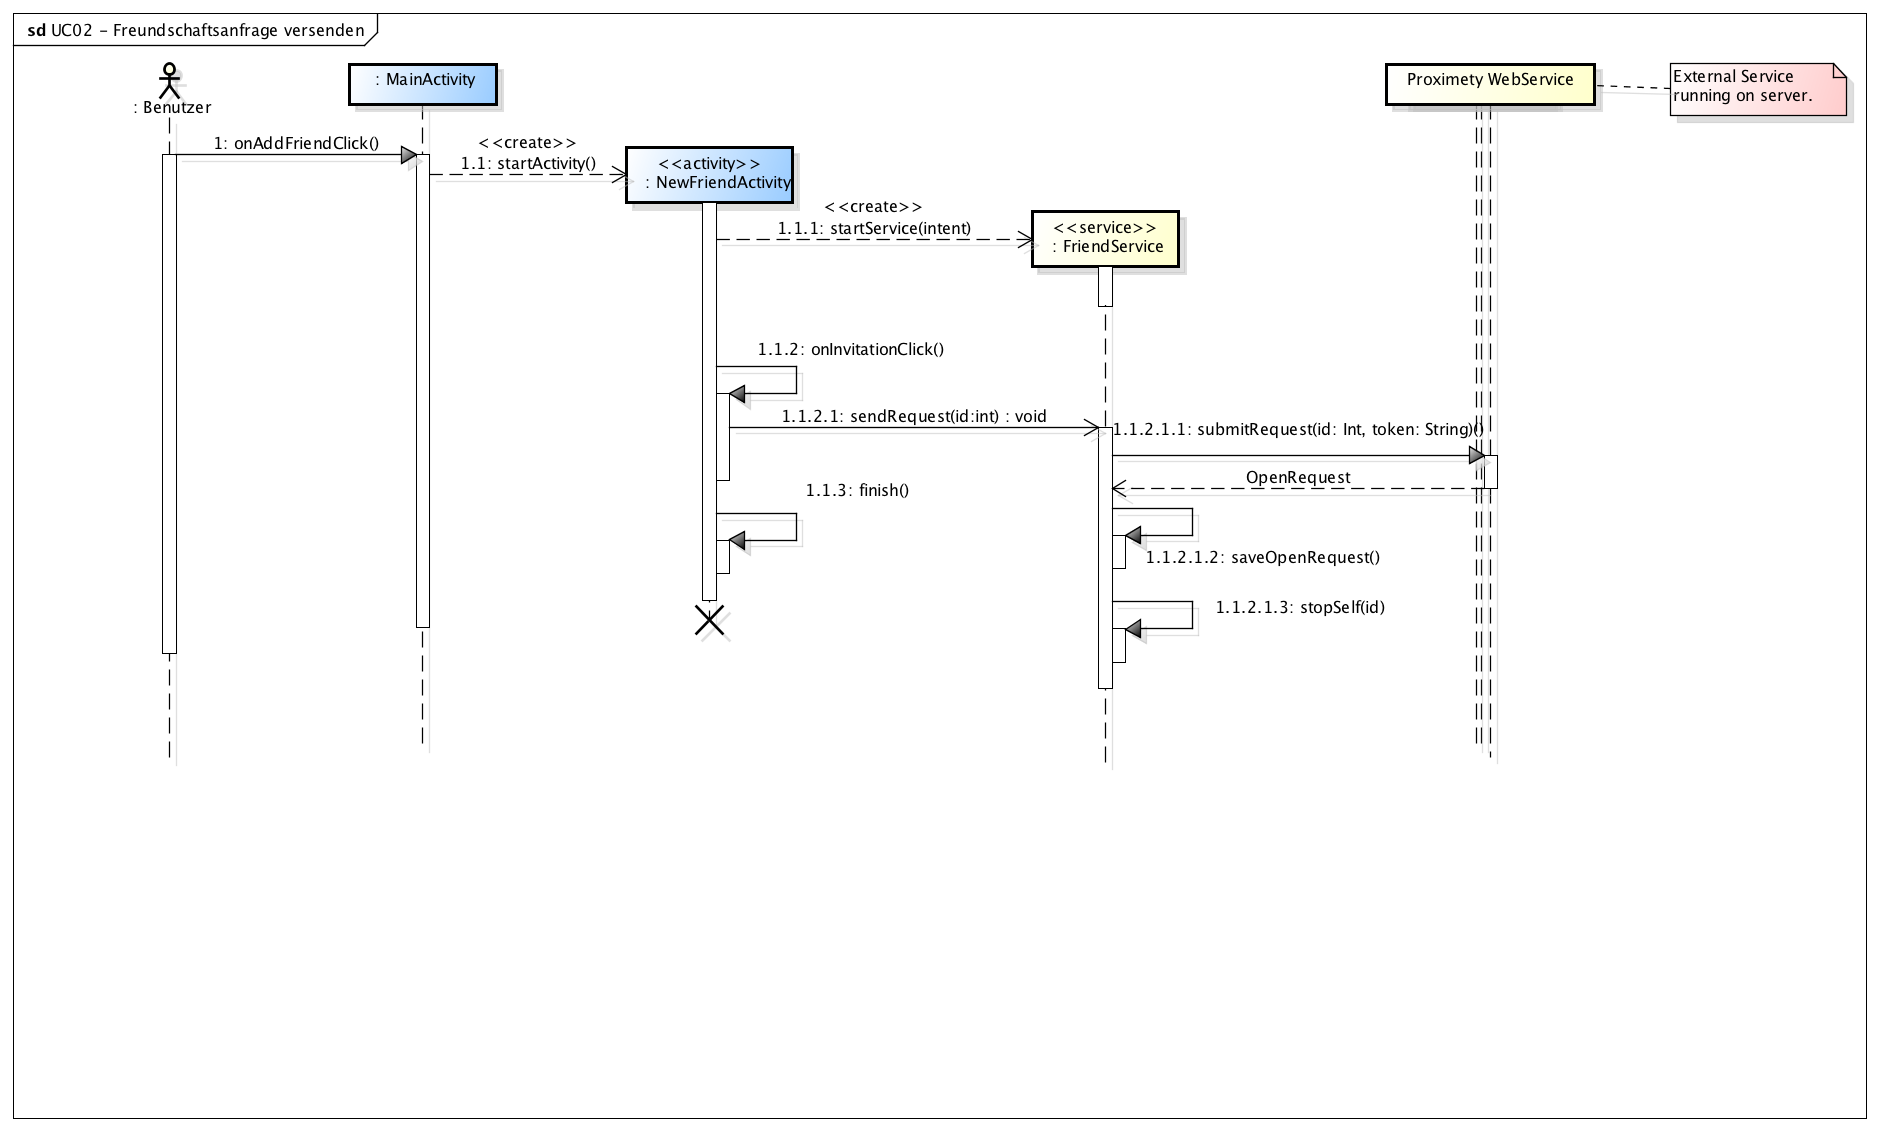
\includegraphics[width=\textwidth]{architektur/UC02_Freundschaftsanfrage_versenden}
	\caption{Sequenzdiagramm Freundschaftsanfrage versenden}
	\label{fig:UC02_Freundschaftsanfrage_versenden}
\end{figure}

\FloatBarrier
\subsection{Sequenzdiagramm Freundschaft aufloesen}
Das Sequenzdiagramm in Abbildung~\ref{fig:UC03_Freundschaft_aufloesen} visualisiert den Prozess, welcher in UC03 beschrieben ist.
\begin{figure}[H]
	\centering
		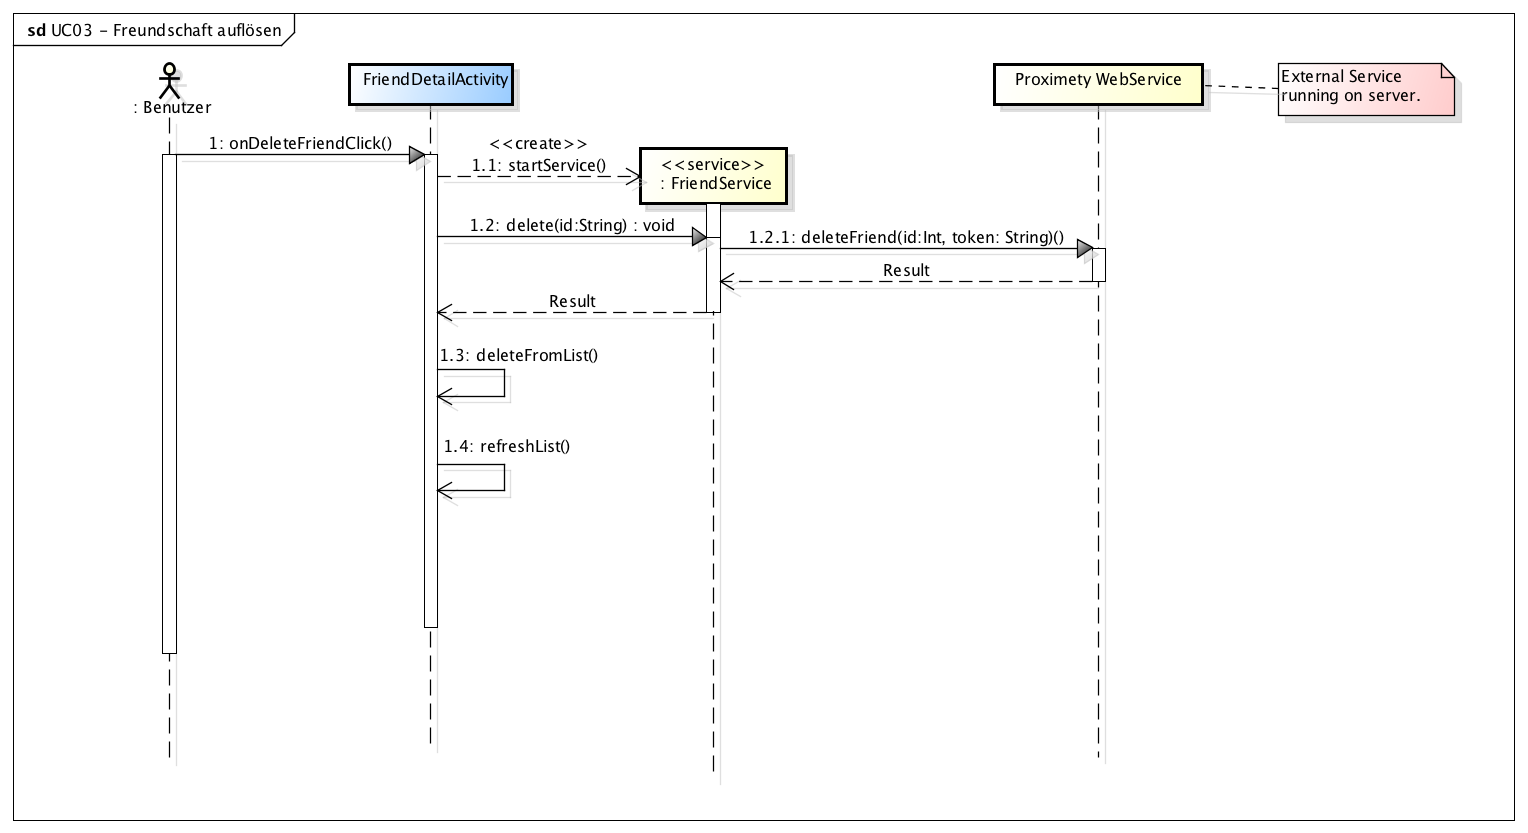
\includegraphics[width=\textwidth]{architektur/UC03_Freundschaft_aufloesen}
	\caption{Sequenzdiagramm Freundschaft aufloesen}
	\label{fig:UC03_Freundschaft_aufloesen}
\end{figure}

\FloatBarrier
\subsection{Sequenzdiagramm Aktueller Standort eines Freundes abfragen}
Das Sequenzdiagramm in Abbildung~\ref{fig:UC04_Aktueller_Standort_eines_Freundes_abfragen} visualisiert den Prozess, welcher in UC04 beschrieben ist.
\begin{figure}[H]
	\centering
		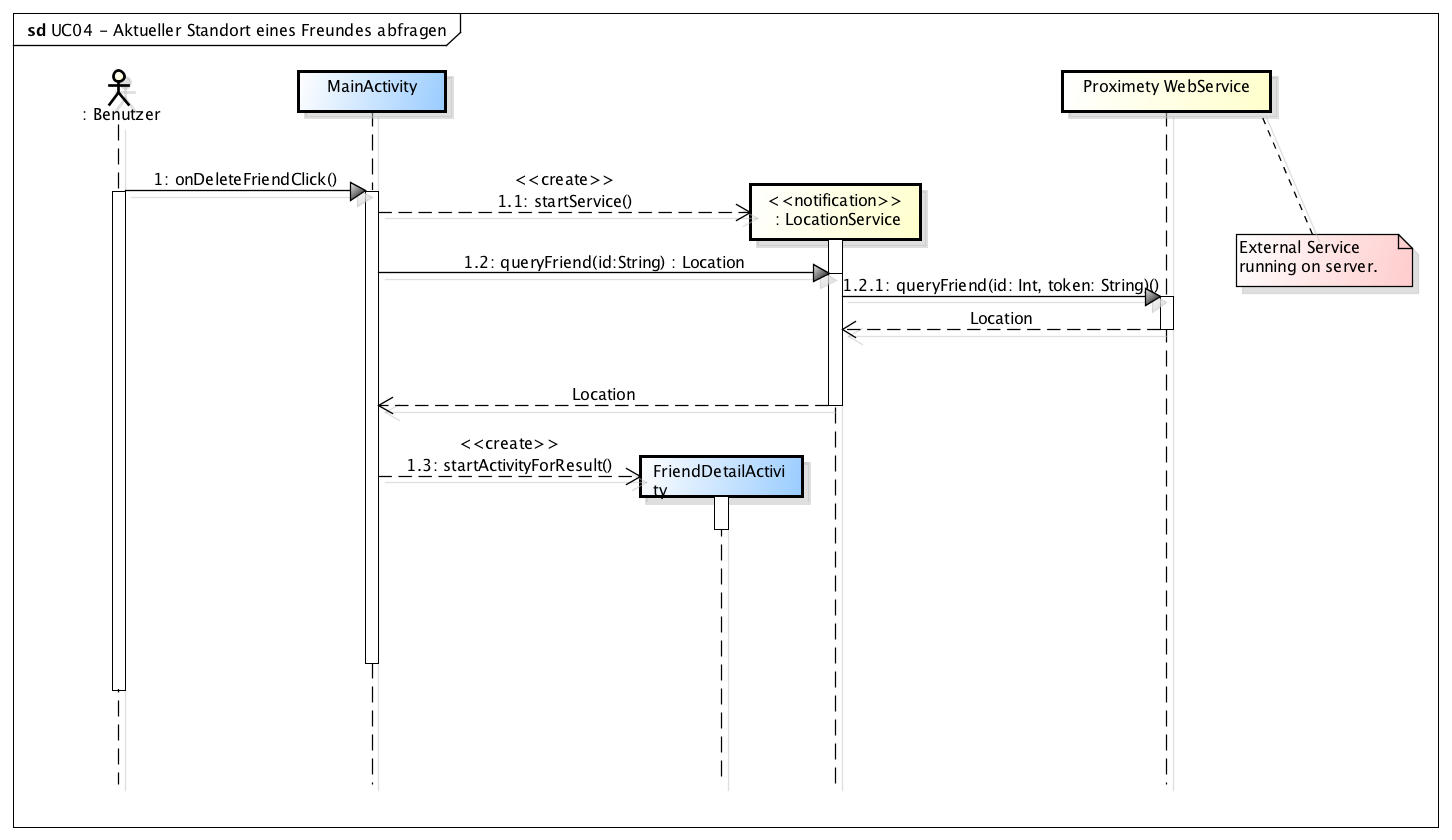
\includegraphics[width=\textwidth]{architektur/UC04_Aktueller_Standort_eines_Freundes_abfragen}
	\caption{Sequenzdiagramm Aktueller Standort eines Freundes abfragen}
	\label{fig:UC04_Aktueller_Standort_eines_Freundes_abfragen}
\end{figure}

\FloatBarrier
\subsection{Sequenzdiagramm Proximety Alarm}
Das Sequenzdiagramm in Abbildung~\ref{fig:UC05_Proximity_Alarm} visualisiert den Prozess, welcher in UC05 beschrieben ist.
\begin{figure}[H]
	\centering
		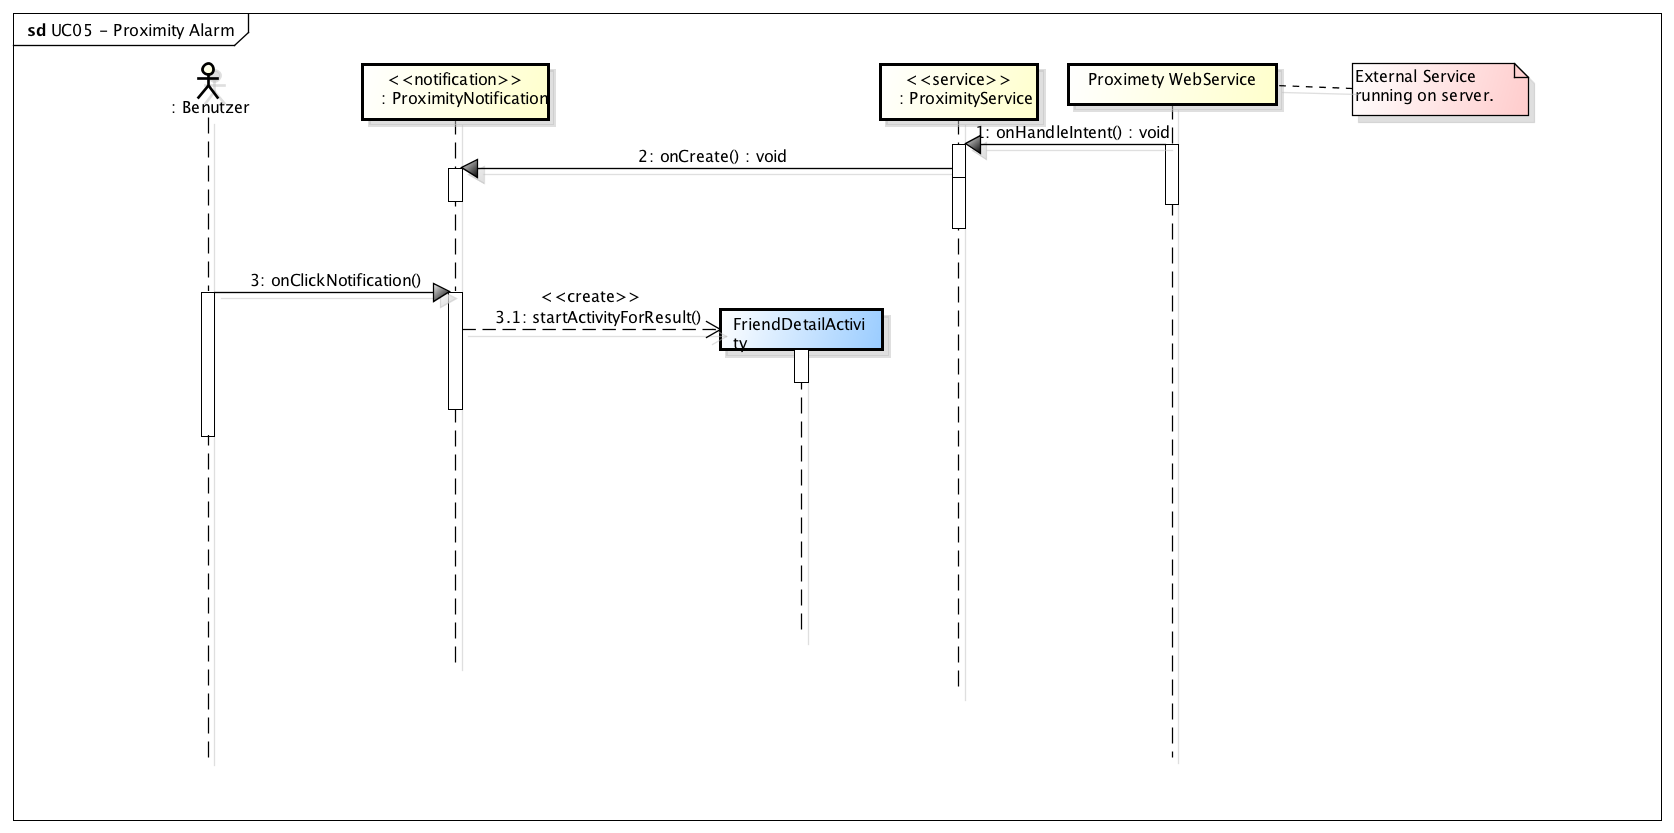
\includegraphics[width=\textwidth]{architektur/UC05_Proximity_Alarm}
	\caption{Sequenzdiagramm Proximety Alarm}
	\label{fig:UC05_Proximity_Alarm}
\end{figure}

\FloatBarrier
\subsection{Sequenzdiagramm Freund kontaktieren}
Das Sequenzdiagramm in Abbildung~\ref{fig:UC06_Freund_kontaktieren} visualisiert den Prozess, welcher in UC06 beschrieben ist.
\begin{figure}[H]
	\centering
		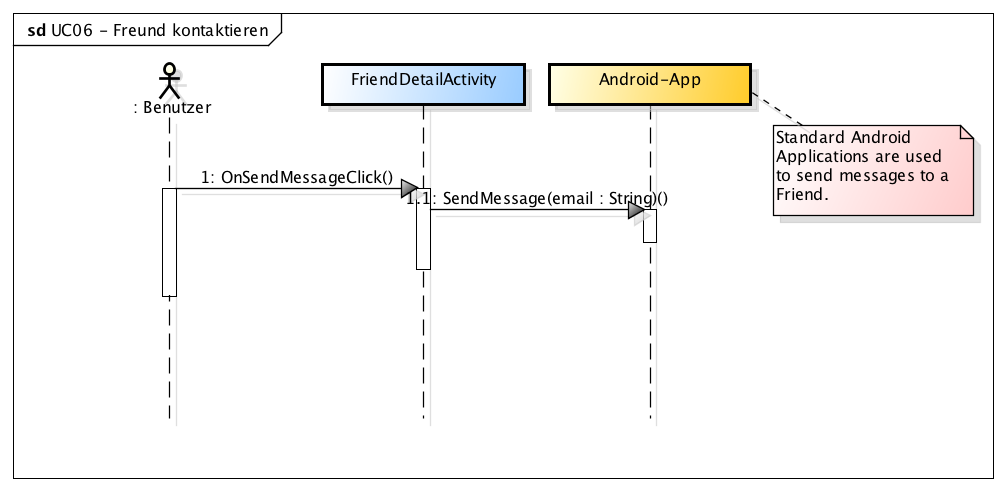
\includegraphics[width=\textwidth]{architektur/UC06_Freund_kontaktieren}
	\caption{Sequenzdiagramm Freund kontaktieren}
	\label{fig:UC06_Freund_kontaktieren}
\end{figure}

\FloatBarrier
\subsection{Sequenzdiagramm Freundspezifische Einstellungen anpassen}
Das Sequenzdiagramm in Abbildung~\ref{fig:UC07_Freund_Spezifische_Einstellungen_anpassen} visualisiert den Prozess, welcher in UC07 beschrieben ist.
\begin{figure}[H]
	\centering
		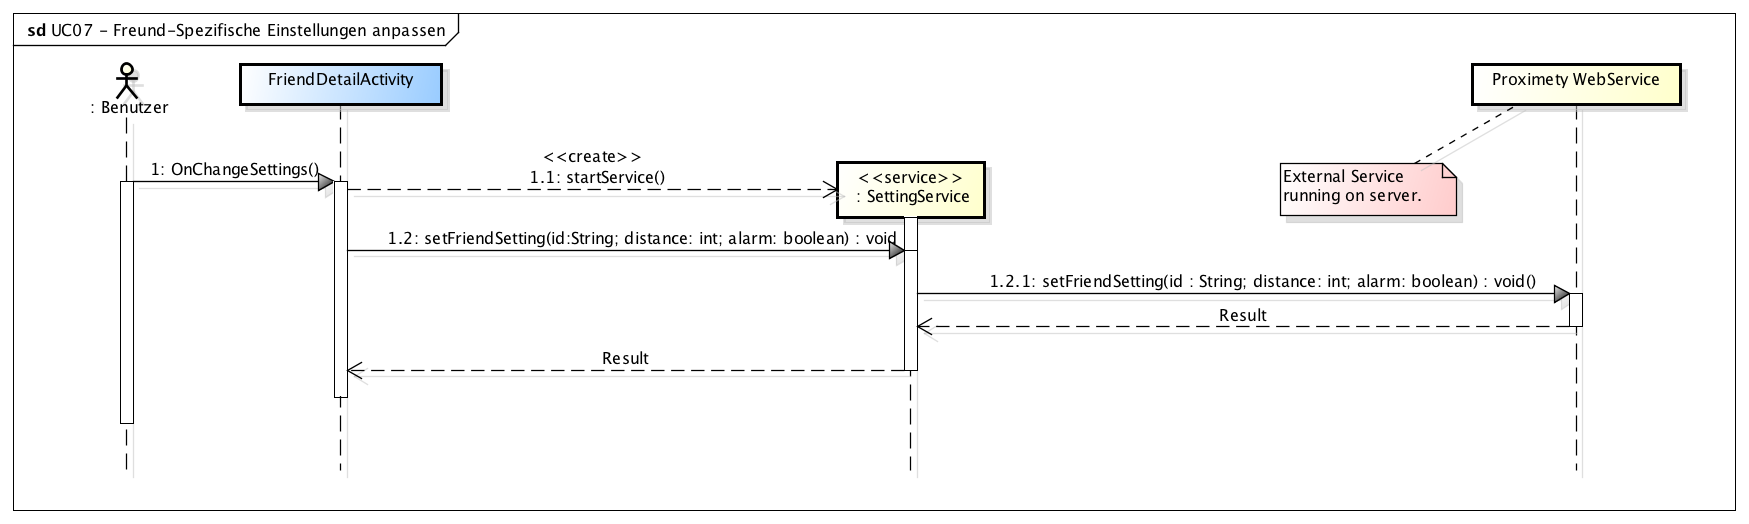
\includegraphics[width=\textwidth]{architektur/UC07_Freund_Spezifische_Einstellungen_anpassen}
	\caption{Sequenzdiagramm Freundspezifische Einstellungen anpassen}
	\label{fig:UC07_Freund_Spezifische_Einstellungen_anpassen}
\end{figure}

\FloatBarrier
\subsection{Sequenzdiagramm Allgemeine App-Einstellungen vornehmen}
Das Sequenzdiagramm in Abbildung~\ref{fig:UC08_Allgemeine_App_Einstellungen_vornehmen} visualisiert den Prozess, welcher in UC08 beschrieben ist.
\begin{figure}[H]
	\centering
		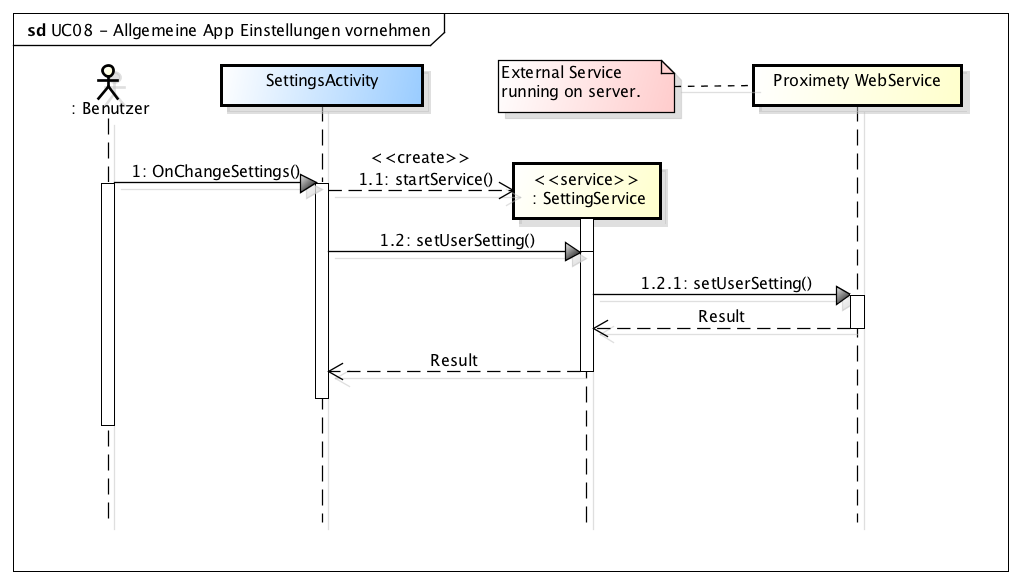
\includegraphics[width=\textwidth]{architektur/UC08_Allgemeine_App_Einstellungen_vornehmen}
	\caption{Sequenzdiagramm Allgemeine App-Einstellungen vornehmen}
	\label{fig:UC08_Allgemeine_App_Einstellungen_vornehmen}
\end{figure}